% -*- TeX-master: "../dipole_ilya_paper.tex" -*-
\section{Fabrication}
% \red{natural to couple capacitively} \red{Thickness of aluminium size of chip }

% \red{Glued to a pcb and bonded with gold wires, connectio input and output to coax lines.}

\begin{figure}[h]
  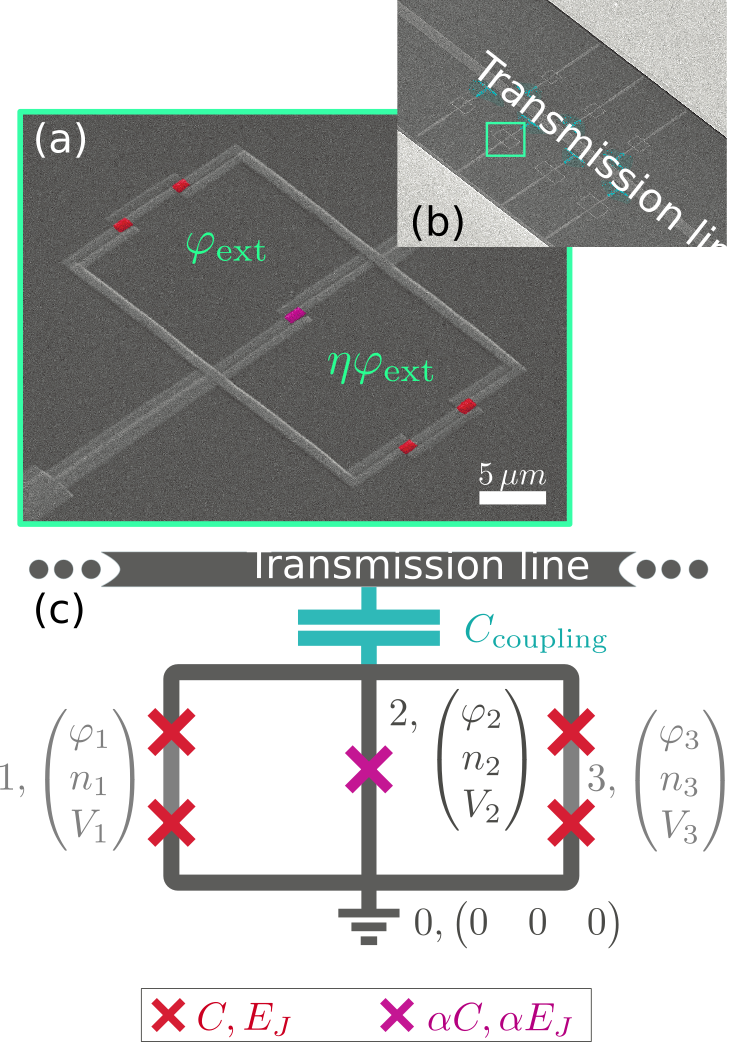
\includegraphics[height=10.5cm]{fig1}
  \caption{\small \textbf{Geometry of a twin qubit:}  a) Scanning electron microscope image of
    the qubit flux with phase biases $ \varphi $,  $ \eta\varphi $ applied to it's superconducting loops. The
    repeated line  structures are the by-product  of the double-angle evaporation  of aluminum
    that creates the Al-AlO$_x$-Al  JJs highlighted in red and pink; b) Each  of the qubits is
    coupled  to the  transmission line  with a  T-shaped  capacitor; c)  The twin  qubit is  a
    symmetrical arrangement of two individual flux qubits (as described in \cite{orlando1999})
    sharing the central  JJ.  Islands are labeled  with a Cooper pair  occupation n$_i$, phase
    $\varphi_i$ and voltage V$_i$, with the ground setting a reference of 0 for all three variables.
    JJs  (marked with  crosses)  mediate  capacitive and  Josephson  interactions between  the
    islands.    The   central  junction   has   a   capacitance   of   $\alpha$C  and   an   energy
    $ \alpha$E$_{J}$, compared with the C$_J$, E$_J$ values of the outside ones.}
  \label{fig:setup}
\end{figure}

%% Describe fabrication
\noindent The qubits and transmission line are fabricated on an undoped 100 silicon substrate,
which is pre-patterned with  10\,nm NiCr\,-\,90\,nm Au ground planes and  markers. We begin by
cleaning the wafer  for $\sim$~10 minutes at  60\,C in acetone rinsing in  de-ionized water.  Two
layers of electron resist are sequentially spun  and post baked (3\,minutes at 60\,C) onto the
wafer:  {Copolymer 13\%},  700\,nm;  ZEP520a:Anisol  2:1, 60\,nm.   We  use  an electron  beam
lithographer  to  expose  the  resist  using  a 30\,kV,  10\,pA  beam  delivering  a  dose  of
$ 70\,\mu $C/cm$^2$.  We develop the pattern in Pylxylen for 35\,seconds followed by a 5\,minute
submersion in  Isopropanol:H$_2$0 93:7 and rinse  in pure Isopropanol.  Shadow  evaporation of
aluminum in a Plassys \cite{wu2013} simultaneously deposits the JJs and the transmission line.
Dry etching  with argon removes oxide  layers for good  galvanic contact to the  gold pattern,
and, maintaining  high vacuum, we  deposit 20\,nm  of Al and  perform static oxidation  for 10
minutes at 0.3\,mBar  to generate the intermediate  AlO$_x$ insulating barrier for  the JJ.  A
second 30\,nm layer of Al completes the process.

These steps give us the 5-JJ structure of  the twin qubits. Qubits are capacitively coupled to
the  transmission line  through and  T-shaped capacitors  them to  the transmission  line, see
Fig.~\ref{fig:setup}.   Each  JJ has  an  a  area  of \iunit{400\times200}{nm$^2$}.   The  coplanar
transmission line  with impedance $  Z_{0} \sim 50\,\Omega  $ runs to  the opening between  the ground
planes in the center of the chip.


We  bond the  sample  chip  to a  printed  circuit board  and  mount it  on  a  holder with  a
niobium-coil magnet on  the 13\,mK stage of a dilution  refrigerator.  A superconducting cover
is used to  shield the holder from stray  magnetic fields. The RF lines running  to the sample
have attenuators, -50\,dBm on the 50K stage,  -30\,dBm on the 4\,K stage, thermalize the input
lines. We  attach a circulator  on the  output line for  isolation. The transmitted  signal is
amplified by  +35\,dBm on  the 4K  stage and  by +35\,dBm  at room  temperature.  This  set of
attenuators and  amplifiers facilitate power  conversion between the laboratory  equipment and
qubit microwaves.  We surround  each temperature stage of the system  with a reflective cover,
that thermally shields from higher  stages.  Prior to performing characterization measurement,
we took the microwave transmission spectrum with  the qubit detuned, and corrected all further
measurements by the background transmission profile.

In this  experiment did  not to go  to the depths  of chemical  and physical treatment  of the
substrate  surface   to  remove  two-level   system  defects   in  the  silicon   oxide  layer
\cite{earnest2018} or employing infra-red filters  to eliminate stray light during measurement
\cite{barends2011}. Rather  we concentrate  on reveling  the intrinsic  potential of  the twin
qubit design and the weaknesses that will have to be addressed in the future.

%%% Local Variables:
%%% mode: latex
%%% TeX-master: "../dipole_ilya_paper"
%%% End:
